\documentclass[5p,sort&compress]{elsarticle}

\usepackage{amssymb}    % Mathematical symbols
\usepackage{amsmath}    % More options for mathematics
\usepackage{subfigure}  % More options for figures
\usepackage{epstopdf}   % Convert eps to pdf
\usepackage[separate-uncertainty=true]{siunitx}   % Proper formatting of units in math mode
\usepackage{color}      % Supports text color if needed
\usepackage{soul}       % https://ctan.org/pkg/soul
\usepackage{lmodern}    % Loading fonts
\usepackage{hyperref}   % To insert clickable references/urls
\usepackage{listings}   % To input code in the text
\usepackage{amsmath}
\usepackage{amsmath}
\usepackage{amssymb}
\usepackage{graphicx}
\usepackage{epstopdf}
\usepackage{booktabs}
\setlength{\parskip}{2em}
\newcommand{\stirlingii}{\genfrac{\{}{\}}{0pt}{}}

% Choose the style of the reference list (do not change)
\bibliographystyle{elsarticle-num}

\journal{ifding/learning-notes}

% Begin the document

\begin{document}

\begin{frontmatter}
    \title{AutoEncoder}
    \author{ifding}
    
    \begin{abstract}
        Probabilistic PCA, Variational AutoEncoder, ELBO surgery
    \end{abstract}


\end{frontmatter}

%% How to make a heading and divide the documents into different sections

\section{Probabilistic PCA}

Principal Component Analysis (known as PCA) is a technique used for dimension-
ality reduction, lossy data compression and data visualization. PCA is a technique that can be analyzed from two different points of view: linear algebra and probability. One of Probabilistic PCA is that it can be used as simple generative model.

PCA finds the principal components of data, or in other words, it finds the features, the directions where there is the most variance. Given a dataset $\mathbf{X}=\{\mathbf{x}^{(i)}\}_1^N$ with dimensionality $D_x$, the main idea beind PCA is to obtain a subspace (called the principal-component subspace) with dimension $D_z$, being $D_z \ll D_x$. So that each $\mathbf{x}^{(i)}$ is represented with a $\mathbf{z}^{(i)}$ (latent variable) in the best possible way. It's possible to recover $\mathbf{x}^{(i)}$ from $\mathbf{z}^{(i)}$.
\begin{equation}
\boldsymbol{x}^{(i)} \in \Re^{D_{x}} \rightarrow \boldsymbol{z}^{(i)} \in \Re^{D_{z}}
\end{equation}

The probabilistic PCA is a maximum likelihood solution of a probabilistic latent variable model in which all marginal and conditional distributions are Gaussian. The likelihood function to be maximized is expressed as:
\begin{equation}
p(\boldsymbol{x})=\int p(\boldsymbol{x} | z) p(z) d z
\end{equation}

As all distributions are Gaussian, the probability distribution of $\boldsymbol{x}$ can be expressed as $p(\boldsymbol{x}) = N(\boldsymbol{x} | \boldsymbol{\mu}, \boldsymbol{C})$, where the covariance matrix is $\boldsymbol{C} = \boldsymbol{W}\boldsymbol{W}^T + \sigma^2$. Therefore, the parameters of the model are the $D_x \times D_z$ matrix $\boldsymbol{W}$, the $D_x$ dimensional vector $\boldsymbol{\mu}$ and the scalar $\sigma^2$.

The optimal values of the parameters are obtained using Maximum Likelihood Estimation (MLE), maximizing the log-likelihood $log p(x)$.
\begin{equation}
\log p\left(\boldsymbol{x} | \boldsymbol{W},\boldsymbol{\mu}, \sigma^{2}\right)=\sum_{i=1}^{N} \log p\left(\boldsymbol{x}^{(i)} | \boldsymbol{W}, \boldsymbol{\mu}, \sigma^{2}\right)
\end{equation}

The optimization can be computed in a closed form or using the EM algorithm. By closed form, the derivative of $\log p\left(\boldsymbol{x} | \boldsymbol{W}, \boldsymbol{\mu},\sigma^{2}\right)$ with respect to each parameter is computed and equal to 0 to obtain the optimal values, namely $\boldsymbol{\mu}_{ML}$, $\boldsymbol{W}_{ML}$ and $\sigma^2_{ML}$.

The optimal mean $\boldsymbol{\mu}_{ML}$ is the sample mean of the data:
\begin{equation}
\boldsymbol{\mu}_{ML}=\sum_{i=1}^{N} \boldsymbol{x}^{(i)}=\bar{\boldsymbol{x}}
\end{equation}

The $\sigma^2_{ML}$ represents the average variance associated with the discarded dimensions.
\begin{equation}
\sigma_{M L}^{2}=\frac{1}{D_{x}-D_{z}} \sum_{i=D_{z}+1}^{D_{x}} \lambda_{i}
\end{equation}

The generation phase comprises two steps. First, the variable $\boldsymbol{z}$ is sampled from a priori known distribution $p(\boldsymbol{z})$. Then, new data samples are drawn from $p(\boldsymbol{x}|\boldsymbol{z}) = N(\boldsymbol{x}|\mu(\boldsymbol{z}), \sigma^2 \boldsymbol{I})$ where $\mu(\boldsymbol{z}) = \boldsymbol{W}\boldsymbol{z} + \boldsymbol{\mu}$. This process is shown in figure~\ref{fig:PCA}.

\begin{figure}[ht]
     \centering
     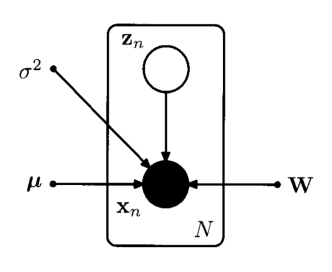
\includegraphics[width = 0.7\linewidth]{figure/PCA_generative.png}
     \caption{PCA generative model.}
     \label{fig:PCA}
\end{figure}

This is a simple case of a generative model where the relation between the latent and the predictive variables is linear:
\begin{equation}
\boldsymbol{x} \sim \boldsymbol{W} z+\boldsymbol{\mu}+\boldsymbol{\epsilon}
\end{equation}


\section{Variational AutoEncoder (VAE)}

The VAE is a type of generative model, which is able to generate realistic data and obtain meaningful latent representations of the input. To achieve this, VAE is based on Bayesian inference. VAE models an approximation of the underlying probability distribution of input data $p(x)$ through a latent variable $z$. VAE can be understood as a non-linear Probabilistic PCA where the non-linearity is introduced using neural networks.
\begin{equation}
\begin{aligned}
\text { Probabilistic } P C A: \quad p(x | z)=N\left(W z+\mu, \sigma^{2} I\right) \\ {\qquad V A E: \quad p_{\theta}(x | z)=N\left(\mu_{\theta}(z), \sigma^{2} I\right)}
\end{aligned}
\end{equation}

What's a variational autoencoder? It's an autoencoder, with a random variable $z$ defined in the latent space, that tries to maximize a lower bound of the data log-likelihood. 

\begin{figure}[ht]
     \centering
     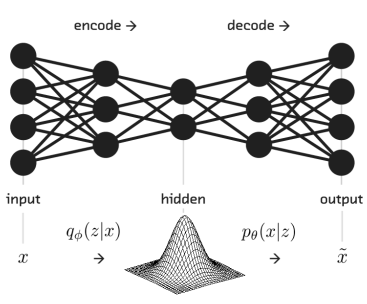
\includegraphics[width = 0.8\linewidth]{figure/probabilistic_vae.png}
     \caption{Probabilistic view of VAE.}
     \label{fig:vae}
\end{figure}

The VAE is composed of two networks as shown in Figure~\ref{fig:vae} and Figure~\ref{fig:graphical}. The encoder or inference network (parameterized by $\phi$) maps the input data into a latent representation that contains important attributes of the data. This latent representation is then mapped, through the decoder of generative network (parameterized by $\theta$), into the reconstructed data.

\begin{figure}[ht]
     \centering
     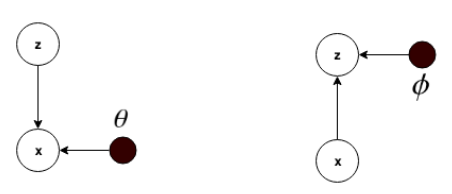
\includegraphics[width = \linewidth]{figure/graphical_vae.png}
     \caption{Graphical models for the VAE showing the generative model (left) and the inference model (right).}
     \label{fig:graphical}
\end{figure}

The main characteristic of VAE is that the latent representation of the input is motivated to be similar to a known distribution. The usual choice is to define the prior distribution $p(z) = N(z|0, \boldsymbol{I})$. In this way, if the latent variable is distributed similarly to $N(z|0, \boldsymbol{I})$ and it holds the correct information about the input data, it's possible to obtain samples from $z$ and then generate realistic data.

Here are some important points about VAE:
\begin{itemize}
\item Similar inputs will have similar representations in the latent space.
\item The dimensions of the latent variable $z$ should be smaller than the dimension of the input so that it captures only the most important features.
\item VAE builds an approximation of the true distribution of the input: $p_g(\boldsymbol{x}) \approx p(\boldsymbol{x})$.
\item A lower bound of $log p(\boldsymbol{x})$ called ELBO is the funtion that will be optimized.
\item All density functions involved in the training process are prefixed. They are assumed to be Gaussian, it's possible to compute its derivatives and use optimization techniques.
\end{itemize}


\subsection{Objective}
Variational autoencoders approximately maximize the density function $p(\boldsymbol{x})$ of the training set according to the formula:
\begin{equation}
p(\boldsymbol{x})=\int p(\boldsymbol{x} | z) p(z) d z
\end{equation}
However, it's not possible to have infinite samples of $z$ to compute the integral, the equation is intractable and there will be losses.  The objective function of the VAE, the Evidence Lower Bound (ELBO):
\begin{equation}
\begin{aligned}
\log p(\boldsymbol{x}) \geq \boldsymbol{E} \boldsymbol{L B O}(\theta, \phi, \boldsymbol{x})= \\ E_{q_{\theta}(z | \mathbf{x})}\left[\log p_{\theta}(\boldsymbol{x} | z)\right]-K L\left(q_{\phi}(z | \boldsymbol{x}) \| p(z)\right)
\end{aligned}
\end{equation}
It's important to mention that only a subset of $\mathbf{X}=\{\mathbf{x}^{(i)}\}_1^N$ samples from the true distribution $p^*(\boldsymbol{x})$ is available. Then, the marginal log likelihood will be approximated as the following equation, which is an unbiased estimator:
\begin{equation}
E_{p^{*}(\boldsymbol{x})}\left[\log p_{\theta}(\boldsymbol{x})\right] \approx \frac{1}{N} \sum_{i=1}^{N} \log p_{\theta}(x^{(i)})
\end{equation}
To reduce the memory needed to compute it, only a mini batch of size M (M $\ll$ N) will be considered at a time, the estimator will remain unbiased but with greater variance.
\begin{equation}
E_{p^{*}(x)}\left[\log p_{\theta}(\boldsymbol{x})\right] \approx \frac{1}{M} \sum_{i=1}^{M} \log p_{\theta}(\boldsymbol{x}^{(i)})
\end{equation}
Finally, the ELBO will be estimated using M samples $\{\mathbf{x}^{(i)}\}_1^M$
\begin{equation}
\frac{1}{M} \sum_{i=1}^{M} \log p_{\theta}\left(\boldsymbol{x}^{(i)}\right) \geq \frac{1}{M} \sum_{i=1}^{M} \boldsymbol{E} \boldsymbol{L} \boldsymbol{B} \boldsymbol{O}(\theta, \phi ; \boldsymbol{x}^{(i)})
\end{equation}

\textbf{1. Dealing with the Integral over z}

To maximize $p(\boldsymbol{x})$, the key idea is to approximate the integral with n samples.
\begin{equation}
p(\boldsymbol{x})=\int p(\boldsymbol{x} | z) p(z) d z = E_{z \sim p(z)}\left[p_{\theta}(\boldsymbol{x} | z)\right]
\end{equation}
Then, if it is possible to obtain n samples from $z$, the equation can be written as:
\begin{equation}\label{eq:p_x}
p(\boldsymbol{x}) \approx \frac{1}{n} \sum_{i=1}^{n} p_{\theta}(\boldsymbol{x} | z^{(i)})
\end{equation}
By convenience, the $log p_{\theta}(\boldsymbol{x}|z)$ will be used instead. It's assumed $p_{\theta}(\boldsymbol{x}|z)$ is distributed as a Gaussian $p_{\theta}(\boldsymbol{x}|z) = N(z|\mu_{\theta}(z), \Sigma)$. Therefore, its log likelihood is proportional to the euclidean distance between $\mu$ and $\boldsymbol{x}$ which is simpler to manipulate analytically.
\begin{equation}
\log p_{\theta}(\boldsymbol{x} | z)=k-\frac{1}{2}\left(\boldsymbol{x}-\mu_{\theta}(z)\right)^{T} \Sigma^{-1}\left(\boldsymbol{x}-\mu_{\theta}(z)\right)
\end{equation}
where
\begin{equation}
k=-\log \left(|\Sigma|^{1 / 2}(2 \pi)^{D_{x} / 2}\right) \quad \Sigma=\sigma^{2} \boldsymbol{I}
\end{equation}
The value of $\sigma^2$ can be chosen, it's desirable to keep it small.

\textbf{2. Inference Network: $q_{\phi}(z|\boldsymbol{x})$}

According to equation~\ref{eq:p_x}, the approximation of $p(\boldsymbol{x})$ is better as the number of samples increases. However, the computation power needed also increases. In practice many values of $z$ do not generate valid data. In conditional probability $p(\boldsymbol{x}|z)$ is close to 0 for the vast majority of $z$. This is why it is defined a family of conditional distributions $q_{\phi}(z|\boldsymbol{x})$ parameterized by $\phi$ that represents the distribution of $z$ for each input datum. Thus, the new approximation is:
\begin{equation}
E_{z \sim q_{\phi}(z | \boldsymbol{x})}\left[\log \left(p_{\theta}(\boldsymbol{x} | z)\right]\right.
\end{equation}
In this way, only values of $z$ that are likely to have produced $\boldsymbol{x}$ are used to compute $p(\boldsymbol{x})$.

\textbf{3. KL Divergence}

The Kullback-Leibler divergence is a measure of how different are two probability functions $p$ and $q$.

For discrete variables it is defines as follows:
\begin{equation}
K L(P(x) \| Q(x))=\sum_{x \in X} P(x) \log \frac{P(x)}{Q(x)}
\end{equation}
For a continuous variable it is defined as follows:
\begin{equation}
KL(p(x) \| q(x))=\int p(x) \log \frac{p(x)}{q(x)} d x=E_{x \sim p(x)}[\log \frac{p(x)}{q(x)}].
\end{equation}

During the VAE optimization, the $K L\left(q_{\phi}(z | \boldsymbol{x}) \| p(z | \boldsymbol{x})\right)$ should be close to 0.
\begin{equation}
K L\left(q_{\phi}(z | \boldsymbol{x}) \| p(z | \boldsymbol{x})\right)=E_{z \sim q_{\phi}}\left[\log q_{\phi}(z | \boldsymbol{x})-\log p(z | \boldsymbol{x})\right]
\end{equation}

\textbf{4. Core Equation}

Applying Bayes rule in $K L\left(q_{\phi}(z | \boldsymbol{x}) \| p(z | \boldsymbol{x})\right)$ and extracting $p(\boldsymbol{x})$ from the expectation because it does not depend on $z$:
\begin{equation}
p(z | x)=\frac{p(x | z) p(z)}{p(x)}
\end{equation}

\begin{equation}
\begin{aligned}
K L\left(q_{\phi}(z | \boldsymbol{x}) \| p(z | \boldsymbol{x})\right)=E_{z \sim q_{\phi}}\left[\log q_{\phi}(z | \boldsymbol{x})-\log p(z | \boldsymbol{x})\right] = \\
E_{z \sim q_{\phi}}\left[\log q_{\phi}(z | \boldsymbol{x})-\log p_{\theta}( \boldsymbol{x} | z) - \log p(z)\right] + \log p(\boldsymbol{x}) =\\
- E_{z \sim q_{\phi}}\left[\log p_{\theta}( \boldsymbol{x} | z)\right] + E_{z \sim q_{\phi}}\left[\log q_{\phi}(z | \boldsymbol{x}) - \log p(z)\right] + \log p(\boldsymbol{x})
\end{aligned}
\end{equation}
It's important to notice that the second term is a KL divergence.  by rearranging terms, the fundamental equation of the VAE is obtained:
\begin{equation}
\begin{aligned}
\log p(\boldsymbol{x})-K L\left(q_{\phi}(z | \boldsymbol{x}) \| p(z | \boldsymbol{x})\right)= \\
E_{z \sim q_{\phi}}\left[\log p_{\theta}(\boldsymbol{x} | z)\right]-K L\left(q_{\phi}(z | \boldsymbol{x}) \| p(z)\right)
\end{aligned}
\end{equation}
Intuitively this equation tell us that the $\log p(\boldsymbol{x})$ minus the encoding error term, is equal to the mean of $\log p_{\theta}(\boldsymbol{x} | z)$ evaluated at $z$ sampled from $q_{\phi}(z|\boldsymbol{x})$ minus an error term.

Because the $p(z|\boldsymbol{x})$ is unknown, it's not possible to calculate $K L\left(q_{\phi}(z | \boldsymbol{x}) \| p(z | \boldsymbol{x})\right)$. This is why this term will be removed from the equation, leading to the loss function of the VAE called ELBO:
\begin{equation}
ELBO(\theta, \phi)=E_{z \sim q_{\phi}}\left[\log p_{\theta}(x | z)\right]-K L\left(q_{\phi}(z | x) \| p(z)\right)
\end{equation}

\begin{itemize}
    \item The $E_{z \sim q_{\phi}}\left[\log p_{\theta}(x | z)\right]$ term represents how good is the reconstrction of the input.
    \item The $K L\left(q_{\phi}(z | x) \| p(z)\right)$ term is a regularizer. In order to maximize the ELBO this term must be small. So this term forces $Q_{\theta}(z|\boldsymbol{x})$ to be similar to $p(z)$.
\end{itemize}


\subsection{ELBO Optimization}

In principle, all the distributions that appear in the ELBO are unknown, so they will be assumed to be Gaussian. This assumption is really convenience because it facilitates the computations since the ELBO will have a closed form. In addition, the Gaussian distribution has the minimal prior structure so it maximizes the entropy.

Then $q_{\theta}(z|\boldsymbol{x})$ is defined as:
\begin{equation}
q_{\phi}(z | \boldsymbol{x})=N\left(\mu_{\phi}(\boldsymbol{x}), \Sigma_{\phi}(\boldsymbol{x})\right)
\end{equation}
And $p(z)$ is defined as:
\begin{equation}
p(z)=N(0, \boldsymbol{I})
\end{equation}
Both $\mu$ and $\Sigma$ are neural networks with parameters $\phi$ that are learnt during training. Moreover, $\Sigma$ is defined as a diagonal matrix so that the $KL(q_{\phi}(z|\boldsymbol{x})||p(z|\boldsymbol{x}))$ has a closed form:
\begin{equation}\
\begin{aligned}
K L\left(N\left(\mu_{\phi}(\boldsymbol{x}), \Sigma_{\phi}(\boldsymbol{x})\right) \| N(0, \boldsymbol{I})\right)= \\ \frac{1}{2}\left[\operatorname{tr}\left(\Sigma_{\phi}(\boldsymbol{x})\right)-D_{z}-\log \operatorname{det}\left(\Sigma_{\phi}(\boldsymbol{x})\right)+\left(\mu_{\phi}(\boldsymbol{x})\right)^{T}\left(\mu_{\phi}(\boldsymbol{x})\right)\right]
\end{aligned}
\end{equation}

The other term involves solving the next integral:
\begin{equation}
E_{z \sim q_{\phi}}\left[\log p_{\theta}(\boldsymbol{x} | z)\right]=\int \log p_{\theta}(\boldsymbol{x} | z) q_{\phi}(z | \boldsymbol{x}) d z
\end{equation}
It is approximated using the Monte Carlo estimator which is short it is an unbiased estimator, its variance is inversely proportional to the number of samples $\sigma^2 \propto \frac{1}{\sqrt{M}}$ and if M is large enough the estimated expectation is similar to the real one.

Then, the Monte Carlo estimator of $E_{z \sim q_{\phi}}\left[\log p_{\theta}(\boldsymbol{x} | z)\right]$ by taking M samples of z, $(z^{(1)}, \ldots, z^{(M)})$, from $q_{\phi}(z|\boldsymbol{x})$ is:
\begin{equation}
E_{z \sim q_{\phi}}\left[\log p_{\theta}(\boldsymbol{x} | z)\right] \approx \frac{1}{M} \sum_{i=1}^{M} \log p_{\theta}(\boldsymbol{x} | z^{(i)})
\end{equation}
\begin{equation}
\begin{aligned}
\log p_{\theta}(\boldsymbol{x} | z^{(i)}) = \\
k-\frac{1}{2}(x-\mu_{\theta}(z^{(i)}))^{T} \Sigma^{-1}(x-\mu_{\theta}(z^{(i)}))
\end{aligned}
\end{equation}
where
\begin{equation}
\Sigma=\sigma^{2} \boldsymbol{I}_{D_{x}} \quad k=-\log \left(|\Sigma|^{1 / 2}(2 \pi)^{D_{x} / 2}\right) \quad|\Sigma|=\left(\sigma^{2}\right)^{D_{x}}
\end{equation}
$\sigma^2$ acts as a weighting factor between the two terms. This parameter depends on the choice of $p_{\theta}(\boldsymbol{x}|z)$. Our choice of $\sigma$ determines how accurately we expect the model to reconstruct $\boldsymbol{x}$. If $\sigma^2$ is small, the first term outweighs the second one forcing $\boldsymbol{x} \approx \mu_{\theta}(z)$.

This formula looks more tractable, but it can not be optimized via backpropagation. Because it's necessary to obtain $z$ samples in an intermediate layer to calculate $\log p_{\theta}(\boldsymbol{x}|z^{(i)})$:
\begin{equation}
x \rightarrow \mu_{\phi}, \Sigma_{\phi} \rightarrow z \sim N\left(\mu_{\phi}, \Sigma_{\phi}\right) \rightarrow \mu_{\theta} \rightarrow x
\end{equation}
The forward pass of this network works fine and, if the output is averaged over many samples of $\boldsymbol{x}$ and z, it produces the correct expected value. However, it's not possible to back-propagate the error through stochastic layers. Sampling is a non-continuous operation and has no gradient.


\subsection{Reparameterization Trick}

In order to obtain the latent representation $z$ of a given observation $\boldsymbol{x}$, it's necessary to sample it from the approximate posterior $q_{\phi}(z|\boldsymbol{x})$. The reparameterization trick consists in moving the sampling from an input layer. This is achieved defining a new input $\epsilon$ that introduces randomness into the model. Now, rather than sampling $z \sim N(\mu_{\phi}, \Sigma_{\phi})$ directly, the sampling is done in $\epsilon \sim N(0, \boldsymbol{I})$ and then $z$ is calculated in a deterministic way $z=\mu_{\phi}(\boldsymbol{x}) + \epsilon \sqrt{\Sigma_{\phi}(\boldsymbol{x})}$:
\begin{equation}
x, \epsilon \rightarrow \mu_{\phi}, \Sigma_{\phi} \rightarrow z=\mu_{\phi}+\sqrt{\Sigma_{\phi}} * \epsilon \rightarrow \mu_{\theta} \rightarrow x
\end{equation}
In this way,backpropagation can be applied to optimize the network parameters.

The sampling of new data is quite straightforward: $z$ is sampled from its prior distribution $p(z) = N(0, \boldsymbol{I})$ and injected into the decoder:
\begin{equation}
z \sim N(0, I) \rightarrow \mu_{\theta}(z) \rightarrow x
\end{equation}


\section{ELBO surgery}

The variational expectation-maximization (EM):
\begin{equation}
p_{\theta}(\boldsymbol{x})=\int p_{\theta}(\boldsymbol{x} | \boldsymbol{z}) p(\boldsymbol{z}) \mathrm{d} \boldsymbol{z}
\end{equation}
where $p(\boldsymbol{z})$ is a prior on latent variables $\boldsymbol{z}=\{z_n\}_{n=1}^N$, $p_{\theta}(\boldsymbol{x} | \boldsymbol{z})$ is a likelihood on observations $\boldsymbol{x}=\{x_n\}_{n=1}^N$ parameterized by $\theta$. The prior and likelihood follow from the generative model.
\begin{equation}
\begin{aligned}
z_{n} \stackrel{\mathrm{iid}}{\sim} \mathcal{N}(0, I) \\
x_{n} | z_{n} \sim \mathcal{N}\left(\mu\left(z_{n} ; \theta\right), \Sigma\left(z_{n} ; \theta\right)\right), \quad n=1,2, \ldots, N
\end{aligned}
\end{equation}
where the mean $\mu\left(z_{n} ; \theta\right)$ and the covariance $\Sigma\left(z_{n} ; \theta\right)$ depend on the latent variable $z_n$ through a neural network with parameters $\theta$.

We write joint densities as products of independent densities.
\begin{equation}
p(\boldsymbol{z})=\prod_{n} p\left(z_{n}\right), \quad p_{\theta}(\boldsymbol{x} | \boldsymbol{z})=\prod_{n} p_{\theta}\left(x_{n} | z_{n}\right)
\end{equation}

The model is fit by maximizing the log evidence lower-bound (ELBO) $\mathcal{L}$,
\begin{equation}
\begin{aligned}
\log p_{\theta}(\boldsymbol{x})=\log \int p_{\theta}(\boldsymbol{z}, \boldsymbol{x}) \mathrm{d} \boldsymbol{z}=\log \int q_{\phi}(\boldsymbol{z} | \boldsymbol{x}) \frac{p_{\theta}(\boldsymbol{z}, \boldsymbol{x})}{q_{\phi}(\boldsymbol{z} | \boldsymbol{x})} \mathrm{d} \boldsymbol{z} \\
\geq \mathbb{E}_{q_{\phi}(\boldsymbol{z} | \boldsymbol{x})} \log \frac{p_{\theta}(\boldsymbol{z}, \boldsymbol{x})}{q_{\phi}(\boldsymbol{z} | \boldsymbol{x})} \triangleq \mathcal{L}(\theta, \phi),
\end{aligned}
\end{equation}

where each term in the variational density $q_{\phi}(\boldsymbol{x} | \boldsymbol{z})=\prod_{n} q_{\phi}\left(z_{n} | x_{n}\right)$ is a Gaussian in which the mean $\mu(x_n ; \phi)$ and covariance $\Sigma\left(x_{n} ; \phi\right)$ depend on the observation $x_n$ through a neural network with free parameters $\phi$.

The variational distribution $q_{\phi}(z_n|x_n)$ acts as a stochastic ``encoder'' from an observation $x_n$ to a distribution on the latent variable $z_n$, and the likelihood $p_{\theta}(x_n | z_n)$ acts as a stochastic ``decoder'' from the latent variable $z_n$ to a distribution on the observation $x_n$.

There are several ways to rewrite the objective $\mathcal{L}(\theta, \phi)$, and each provides its own perspective.


\subsection{Evidence minus posterior KL}

One form of $\mathcal{L}(\theta, \phi)$ emphasizes that the lower bound becomes tighter as the variational distribution better approximates the posterior:
\begin{equation}
\mathcal{L}(\theta, \phi)=\log p_{\theta}(\boldsymbol{x})-\mathrm{KL}\left(q_{\phi}(\boldsymbol{z} | \boldsymbol{x}) \| p_{\theta}(\boldsymbol{z} | \boldsymbol{x})\right)
\end{equation}
Thus we cam improve the ELBO by improving the model log evidence $\log p_{\theta}(\boldsymbol{x})$, through the prior $p(\boldsymbol{z})$ or the likelihood $p_{\theta}(\boldsymbol{x} | \boldsymbol{z})$, or by improving the variational posterior approximation $q_{\phi}(\boldsymbol{z} | \boldsymbol{x})$.

\subsection{Average negative energy plus entropy}

Another way to rewrite the ELBO is as
\begin{equation}
\begin{aligned}
\mathcal{L}(\theta, \phi)=\mathbb{E}_{q_{\phi}(z | \boldsymbol{x})}\left[\log p_{\theta}(\boldsymbol{z}, \boldsymbol{x})\right]+\mathbb{H}\left[q_{\phi}(\boldsymbol{z} | \boldsymbol{x})\right], \\
\mathbb{H}\left[q_{\phi}(\boldsymbol{z} | \boldsymbol{x})\right] \triangleq-\mathbb{E}_{q_{\phi}(\boldsymbol{z} | \boldsymbol{x})} \log q_{\phi}(\boldsymbol{z} | \boldsymbol{x}),
\end{aligned}
\end{equation}
where the log joint $\log p_{\theta}(\boldsymbol{z}, \boldsymbol{x})$ is interpreted as the negative energy in a Boltzmann distribution. Since we choose $(\theta, \phi)$ to maximize the ELBO, this version highlights that a good posterior approximation $q_{\phi}(\boldsymbol{z} | \boldsymbol{x})$ must assign most of its probability mass to regions of low energy (i.e. high joint probability density) while also maximizing the entropy of $q_{\phi}(\boldsymbol{z} | \boldsymbol{x})$.

This perspective is useful in contrasting variational EM with a maximum a-posteriori (MAP) approach; while MAP need only find a single value of $\boldsymbol{z}$ that maximizes the joint density (even if it lies in a region with very low posterior mass), the entropy term in the ELBO prevents $q_{\phi}(\boldsymbol{z}|\boldsymbol{x})$ from collapsing to an atom.


\subsection{Average term-by-term reconstruction minus KL to prior}

Finally, we can write
\begin{equation}
\begin{aligned}
\mathcal{L}(\theta, \phi)=\frac{1}{N} \sum_{n=1}^{N} \mathbb{E}_{q_{\phi}\left(z_{n} | x_{n}\right)}\left[\log p_{\theta}\left(x_{n} | z_{n}\right)\right]- \\
\operatorname{KL}\left(q_{\phi}\left(z_{n} | x_{n}\right) \| p\left(z_{n}\right)\right)
\end{aligned}
\end{equation}
For each observation index $n$, this version has a reconstruction term for the $n$th observation and a KL divergence from each encoding distribution to the prior. This KL-divergence term can be interpreted as a regularizer that ``prune out'' many of the latent dimensions in $\boldsymbol{z}$.


\subsection{Terms of the average encoding distribution}

For the last decomposition, what's a reasonable value for the KL-divergence term? Ideally it would be small, but we do not want it to approach 0 ($q_{\phi}(z_n | x_n) = p(z_n)$), since that would imply that $x_n$ and $z_n$ were almost independent, whereas virtually all of our modeling power comes from strongly coupling $x_n$ to $z_n$. So if the KL term is large, is that a sign of underfitting, overfitting, or neither?

The \textit{average encoding distribution} is defined as
\begin{equation}
q_{\phi}^{\mathrm{avg}}(z) \triangleq \frac{1}{N} \sum_{n=1}^{N} q_{\phi}\left(z | x_{n}\right)
\end{equation}
The \textit{marginal} KL divergence $\operatorname{KL}(q_{\phi}^{\mathrm{avg}}(z) \| p(z))$ is important because, unlike the individual terms $q_{\phi}(z_n | x_n)$, the average encoding distribution $q_{\phi}^{\mathrm{avg}}(z)$ can be made arbitrarily close to the prior $p(z)$ without sacrificing model power. Indeed, if the data are drawn from the model, $x_n \sim p_{\theta}(x)$, and the posterior approximation is accurate, $q_{\phi}\left(z | x_{n}\right) \approx p_{\theta}\left(z | x_{n}\right)$, then for large N we would expect
\begin{equation}
\begin{aligned}
p(z)=\int p_{\theta}(z | x) p_{\theta}(x) \mathrm{d} x=\mathbb{E}_{x \sim p_{\theta}(x)} p_{\theta}(z | x) \approx \\ 
\frac{1}{N} \sum_{n} p_{\theta}\left(z | x_{n}\right) \approx \frac{1}{N} \sum_{n} q_{\phi}\left(z | x_{n}\right)=q_{\phi}^{\mathrm{avg}}(z)
\end{aligned}
\end{equation}

To simplify the notation, we drop parameter subscripts, and it's convenient to treat the index $n$ as a random variable.
\begin{equation}
q(n, z) \triangleq q(n) q(z | n), \quad q(z | n) \triangleq q\left(z | x_{n}\right), \quad q(n) \triangleq \frac{1}{N}
\end{equation}
\begin{equation}
p(n, z) \triangleq p(n) p(z | n), \quad p(z | n) \triangleq p(z), \quad \quad p(n) \triangleq \frac{1}{N}
\end{equation}
where $p(z)$ denotes a standard Gaussian prior density form $z \sim \mathcal{N}(0, I)$, the average encoder distribution $q^{\mathrm{avg}}(z)$ is now simply the marginal $q(z) = \sum_{n=1}^N q(z,n)$.

\begin{equation}
\begin{aligned} \frac{1}{N} \sum_{n=1}^{N} \mathrm{KL}\left(q\left(z_{n} | x_{n}\right) \| p\left(z_{n}\right)\right) =\sum_{n} q(n, z) \log \frac{q(n, z)}{p(n, z)} \\ = q(z) \log \frac{q(z)}{p(z)} + \sum_{n} q(n|z) q(z) \log \frac{q(n|z)}{p(n|z)}\\
=\mathrm{KL}(q(z) \| p(z))+\mathbb{E}_{q(z)}[\mathrm{KL}(q(n | z) \| p(n))] \\ 
= \mathrm{KL}(q(z) \| p(z)) + \mathbb{I}_{q(n, z)}[n, z] \\ =\mathrm{KL}(q(z) \| p(z))+\left(\log N-\mathbb{E}_{q(z)}[\mathbb{H}[q(n | z)]]\right) \end{aligned}
\end{equation}
where $\mathbb{I}_{q(n, z)}[n, z]=\mathbb{E}_{q(n, z)}\left[\log \frac{q(n, z)}{q(n) q(z)}\right]$ denotes the mutual information of $n$ and $z$ in $q(n,z)$, $p(n) = \frac{1}{N}$. The mutual information expression:
\begin{equation}
\begin{aligned}
\mathbb{I}_{q(n, z)}[n, z]=\mathbb{E}_{q(z)}\left[\mathbb{E}_{q(n | z)}\left[\log \frac{q(n | z)}{q(n)}\right]\right]= \\
\log N-\mathbb{E}_{q(z)}[\mathbb{H}[q(n | z)]]
\end{aligned}
\end{equation}

The ELBO can be written in three terms:
\begin{equation}
\begin{aligned}
\mathcal{L}(\theta, \phi)=\underbrace{\left[\frac{1}{N} \sum_{n=1}^{N} \mathbb{E}_{q\left(z_{n} | x_{n}\right)}\left[\log p\left(x_{n} | z_{n}\right)\right]\right.}_{\text {(1) average reconstruction }} \\
- \underbrace{\left(\log N-\mathbb{E}_{q(z)}[\mathbb{H}[q(n | z)]]\right)}_{\text {(2) index-code mutual info. }} \\
- \underbrace{\mathrm{KL}(q(z) \| p(z))}_{\text {(3) marginal KL to prior }}
\end{aligned}
\end{equation}

First, the two terms (1) and (2) are in tension with each other because to get a good average reconstruction score for (1), we typically need each encoding $z_n$ to be specific to its corresponding observation $x_n$ and hence $q(n|z)$ should have low entropy. Term (2) acts as a regularizer, in that it encourages the encodings $q(z|x_n)$ to overlap for distinct observation $n$, but this effect is likely to be weak relative to the reconstruction term (1). (2) is bounded above and below,
\begin{equation}
0 \leq \log N-\mathbb{E}_{q(z)} \mathbb{H}[q(n | z)] \leq \log N
\end{equation}
Empirically, the reconstruction is precise and correspondingly, $q(z|n)$ is concentrated relative to $q(z)$, resulting in (2) is close to its maximum value of $\log N$.

Second, while $q(z)$ appears in all terms, $p(z)$ only appears in (3). Thus when considering choosing priors $p(z)$ to optimize the ELBO, only this term is affected. Observe that we could set (3) to zero without sacrificing model power by simply defining the prior to be $q(z)$. This choice would not be amenable to scalable computation because it is difficult to evaluate (2) in isolation: to normalize $q(n|z)$ at each evaluation requires accessing all N observations (and the normalization also precludes us from making unbiased Monte Carlo estimates). Setting (3) to zero may also be undesirable due to the potential for overfitting or the inability to use the prior to sculpt the latent representation. Because (3) can in principle be set to zero, whenever it is large it indicates a very strong and potentially unwanted regularization effect from the prior.


%\section*{References}
\bibliography{references}

\begin{thebibliography}{9}

\bibitem{pablo}
Sánchez Martín, P., 2018. Unsupervised deep learning research and implementation of variational autoencoders (Bachelor's thesis).

\bibitem{Bishop} 
Bishop, Christopher M. Pattern recognition and machine learning. springer, 2006.

\bibitem{vae}
Kingma, D.P. and Welling, M., 2013. Auto-encoding variational bayes. arXiv preprint arXiv:1312.6114.

\bibitem{hoffman}
Hoffman, M.D. and Johnson, M.J., 2016, December. Elbo surgery: yet another way to carve up the variational evidence lower bound. In Workshop in Advances in Approximate Bayesian Inference, NIPS (Vol. 1).

\end{thebibliography}
\end{document}